\documentclass[11pt, a4paper]{article}
\usepackage{CJKutf8}
\usepackage{amsthm}
\usepackage{ulem}
\usepackage{xcolor}
\usepackage{amsmath}
\usepackage{amssymb}
\usepackage{courier}
\usepackage{geometry}
\usepackage{enumitem}
\usepackage{graphicx}
\usepackage{listings}
\usepackage{algorithm}
\usepackage{algorithmic}
\usepackage{indentfirst}
\usepackage{minted}
\usepackage[toc,page,title,titletoc,header]{appendix} 
%\usepackage{float}
\usepackage[perpage,stable]{footmisc} 
\geometry{left=2.7cm, right=2.7cm, top=3cm, bottom=3cm}


\usepackage{graphics}

\usepackage[colorlinks,linkcolor=black,anchorcolor=blue,citecolor=green,
  %	CJKbookmarks=true,
]{hyperref}
\hypersetup{unicode}

\linespread{1.4}
\usepackage{indentfirst}
\setlength{\parindent}{2em}
\hypersetup{hidelinks}

\renewcommand\thesection{\arabic {section}}
\usepackage{listings}
\lstset{
  numbers=left,
  texcl=true,
  escapechar=`,
  backgroundcolor=\color{lightgray!40!white}, 
  commentstyle=\rm\color{green!30!black},
  basicstyle=\footnotesize\tt,        % the size of the fonts that are used for the code
  breakatwhitespace=false,         % sets if automatic breaks should only happen at whitespace
  breaklines=true,                 % sets automatic line breaking
  captionpos=b,                    % sets the caption-position to bottom
  extendedchars=false,              % lets you use non-ASCII characters; for 8-bits encodings only, does not work with UTF-8
  frame=single,                    % adds a frame around the code
  language=C++,                 % the language of the code
  keywordstyle=\color{blue!70}\bfseries,
  showspaces=false,                % show spaces everywhere adding particular underscores; it overrides 'showstringspaces'
  showstringspaces=false,          % underline spaces within strings only
  showtabs=false,                  % show tabs within strings adding particular underscores
  tabsize=2                       % sets default tabsize to 2 spaces
}

\begin{document}
\begin{CJK*}{UTF8}{gbsn}
  \title{\Huge \bf 2016秋季学期数字逻辑设计大作业报告}
  \author{计算机科学与技术学院\\马玉坤\\1150310618}
  \date{2016年12月22日}
  \maketitle
  \newpage
  \renewcommand{\contentsname}{\textbf{目录}}
  \tableofcontents
\newpage
  \section{引言}
  
  20 世纪末,数字电子技术得到了飞速发展,有力地推动和促进了社会生产力的发展和社会信息化的提高,数字电子技术的应用已经渗透到人类生活的各个方面。从计算机到手机,从数字电话到数字电视,从家用电器到军用设备,从工业自动化到航天技术,都尽可能采用了数字电子技术。
  
  现代电子设计技术的核心是 EDA 技术。EDA(电子设计自动化)技术就是以计算机为工具,在 EDA 软件平台上,对硬件语言 HDL 为系统逻辑描述手段完成的设计文件,自动的完成逻辑编译、逻辑化简、逻辑综合及优化、逻辑仿真,直至对特定目标芯片的适配编译、逻辑映射和编程下载等工作 EDA 的仿真测试技术只需要通过计算机就能对所设计的电子系统从各种不同层次的系统性能特点完成一系列准确的测试与仿真操作,大大提高了大规模系统电子设计的自动化程度。设计者的工作仅限于利用软件方式,即利用硬件描述语言(如 VHDL)来完成对系统硬件功能的描述。EDA 技术使实现,极大地提高了设计效率,缩短了设计周期,节省了设计成本。
  
  今天 EDA 技术已经成为电子设计的重要工具,无论是设计芯片还是设计系统,如果没有 EDA 工具的支持,都将是难以完成的。EDA 工具已经成为现代电路设计工程师的重要武器,正在发挥越来越重要的作用。为了提高自身的实践能力与专业知识应用能力,为了更快地与社会实际和社会需要接轨,这次设计我们小组选择了以汽车尾灯作为设计课题。相信通过此次课题设计将为我更全面更系统更深入地掌握 EDA 技术打下良好们的基础。

  \section{设计目的及要求}

  本次大作业,我选择了汽车尾灯控制器设计。

  \subsection{基础任务}

  设计四种显示模式如下。

  \begin{itemize}
  \item 汽车正向行驶:按下上按钮,所有指示灯熄灭;
  \item 汽车右转弯:按下右按钮或者同时按下上按钮与右按钮,右侧三个指示灯按右循环模式顺序点亮;
  \item 汽车左转弯:按下左按钮或者同时按下上按钮与左按钮,左侧三个指示灯按左循环模式顺序点亮;
  \item 临时刹车:按下下按钮,左右两侧的指示灯同时处于闪烁状态。
  \end{itemize}

  \subsection{附加任务}

  对四种显示模式进行改进,添加了七段数码管的显示。

  \begin{itemize}
  \item 汽车正向行驶:按下上按钮,数码管无显示;
  \item 汽车右转弯:按下右按钮或者同时按下上按钮与右按钮,数码管显示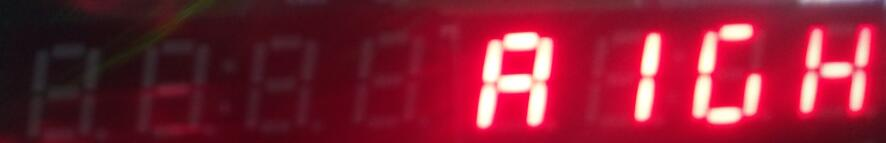
\includegraphics[height=0.5in]{right.jpg};
  \item 汽车左转弯:按下左按钮或者同时按下上按钮与左按钮,数码管显示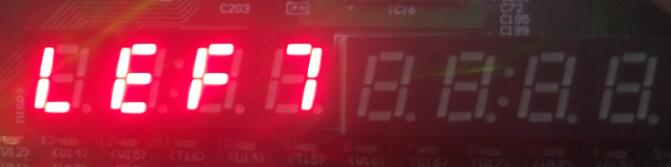
\includegraphics[height=0.5in]{left.jpg};
  \item 临时刹车:按下下按钮,数码管显示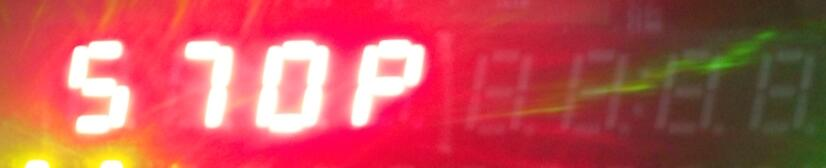
\includegraphics[height=0.5in]{stop.jpg};
  \item 故障状态:其他情况,数码管显示
\includegraphics[height=0.5in]{error.jpg}。
  \end{itemize}

  \section{工作原理}

  为了能够让led灯能够按顺序点亮或者闪烁,就必须要使用小频率的时钟信号,而开发板的E3管脚会输出一个频率为100Mhz的时钟信号。为了获得一个4hz的时钟信号,我使用了一个计数器,会在100MHz信号的上升沿自加1,然后判断是否大于100110001001011010000000,如果大于,就使4hz时钟信号取反,从而产生一个4hz的时钟信号。

  由于Nexys 4 DDR开发板的构造,在同一时间,只能制定若干位七段数码管,显示同样的符号。想要让不同位上的七段数码管同时显示不同的符号,就要利用人眼的“视觉暂留”效应。设置一个高频率(除了频率为4hz的信号,我又生成了频率为1Khz的信号)的信号,在一个周期内,让一位七段数码管显示对应的符号,然后在下一个周期内,让另一位七段数码管显示对应的符号,这样就造成了不同位显示不同符号的“错觉”。

  \section{实现}

  本次作业,我只使用了light这一个模块,负责所有功能。

  同时,我使用了go\_staight、turn\_left、turn\_right、go\_back、output\_error等五个过程来分别来实现向前、左转、右转、刹车、错误输出的功能,以使整个程序结构清晰可读。

  \subsection{实体与端口}
  
  \begin{minted}{vhdl}
Entity light Is
port (
		btn : in STD_LOGIC_VECTOR(4 downto 0);   --五个方向按钮
		led : out STD_LOGIC_VECTOR(15 downto 0); --led控制
		clk : in STD_LOGIC;                      --1MHz信号
		seg : out STD_LOGIC_VECTOR(6 downto 0);  --数码管的七臂
		AN : out STD_LOGIC_VECTOR(7 downto 0)    --八位数字使能
	);
end light;
  \end{minted}

  \subsection{信号定义}

  \begin{minted}{vhdl}
Signal led_int : STD_LOGIC_VECTOR(15 downto 0) := (others => '0');
signal sseg_i : STD_LOGIC_VECTOR(2 downto 0) := (others=>'0');

signal clk4hz : std_logic := '0';
signal clk4hz_n: STD_LOGIC_VECTOR(23 downto 0) := "100110001001011010000000";
signal clk4hz_i : STD_LOGIC_VECTOR(23 downto 0) := (others => '0');

signal clk1khz : std_logic := '0';
signal clk1khz_n : std_logic_vector(16 downto 0) := "11000011010100000";
signal clk1khz_i : std_logic_vector(16 downto 0) := "11000011010100000";
  \end{minted}

  \subsection{主过程}

  \begin{minted}{vhdl}
begin
        led <= led_int;

        --分频
        process(clk, clk4hz) begin
        if rising_edge(clk) then
            clk4hz_i <= clk4hz_i + 1;
            if (clk4hz_i >= clk4hz_n) then
                clk4hz <= not clk4hz;
                clk4hz_i <= (others => '0');
            end if;
            
            clk1khz_i <= clk1khz_i + 1;
            if (clk1khz_i >= clk1khz_n) then
                clk1khz <= not clk1khz;
                clk1khz_i <= (others => '0');
            end if;
        end if;
        end process;

        --设置计数器,调整数码管点亮的位(一次显示一位)
        process(clk1khz) begin
        if rising_edge(clk1khz) then
            sseg_i <= sseg_i + 1;
            if sseg_i = "101" then
                sseg_i <= "000";
            end if;
        end if;
        end process;
        

        --检查按钮的按下情况,进行不同操作
        process (btn) begin
            if btn = "00010" then
                AN <= "11111111";
                go_straight(led_int);
            elsif btn = "00100" or btn = "00110" then 
                turn_left(led_int, AN, seg, clk4hz, sseg_i);
            elsif btn = "01000" or btn = "01010" then
                turn_right(led_int, AN, seg, clk4hz, sseg_i);
            elsif btn = "10000" then
                go_back(led_int, AN, seg, clk4hz, sseg_i);
            elsif btn = "00000" then
                AN <= "11111111";
                led_int <= (others => '1');
            else 
                output_error(AN, seg, sseg_i);
            end if;
        end process;
            
end behavior;

  \end{minted}

  \subsection{左转}

  \begin{minted}{vhdl}
procedure turn_left (signal va : inout STD_LOGIC_VECTOR(15 downto 0);
                     signal an : out STD_LOGIC_VECTOR(7 downto 0);
                     signal seg : out STD_LOGIC_VECTOR(6 downto 0);
                     signal clk4hz : in STD_LOGIC;
                     signal sseg_i : in STD_LOGIC_VECTOR(2 downto 0)) is
begin
    va(12 downto 0) <= (others => '0');
    case sseg_i(2 downto 0) is
        when "000" =>
            an <= "01111111" ;
            seg <= "1000111";
        when "001" =>
            an <= "10111111";
            seg <= "0000110";
        when "010" =>
            an <= "11011111";
            seg <= "0001110";
        when "011" =>
            an <= "11101111";
            seg <= "1111000";
        when others =>
            an <= "11111111";
    end case;
    
    if rising_edge(clk4hz) then
        case va(15 downto 13) is
            when "100" =>
                va(15 downto 13) <= "001";
            when "010" =>
                va(15 downto 13) <= "100";
            when "001" =>
                va(15 downto 13) <= "010";
            when others =>
                va(15 downto 13) <= "100";
        end case;
    end if;
end;

  \end{minted}

  \subsection{右转}

  \begin{minted}{vhdl}
procedure turn_right (signal va : inout STD_LOGIC_VECTOR(15 downto 0);
                     signal an : out STD_LOGIC_VECTOR(7 downto 0);
                     signal seg : out STD_LOGIC_VECTOR(6 downto 0);
                     signal clk4hz : in STD_LOGIC;
                     signal sseg_i : in STD_LOGIC_VECTOR(2 downto 0)) is
begin
    va(15 downto 3) <= (others => '0');
    case sseg_i(2 downto 0) is
        when "000" =>
            an <= "11110111" ;
            seg <= "0001000";
        when "001" =>
            an <= "11111011";
            seg <= "1111001";
        when "010" =>
            an <= "11111101";
            seg <= "1000010";
        when "011" =>
            an <= "11111110";
            seg <= "0001001";
        when others =>
            an <= "11111111";
    end case;
    if rising_edge(clk4hz) then
        case va(2 downto 0) is
            when "001" =>
                va(2 downto 0) <= "100";
            when "010" =>
                va(2 downto 0) <= "001";
            when "100" =>
                va(2 downto 0) <= "010";
            when others =>
                va(2 downto 0) <= "001";
        end case;
    end if;
end;
  \end{minted}

  \subsection{前进}

  \begin{minted}{vhdl}
procedure go_straight (signal va : inout STD_LOGIC_VECTOR(15 downto 0)) is
begin
    va <= (others => '0');
end;
  \end{minted}

  \subsection{刹车}

  \begin{minted}{vhdl}
procedure go_back (signal va : inout STD_LOGIC_VECTOR(15 downto 0);
                   signal an : out STD_LOGIC_VECTOR(7 downto 0);
                   signal seg : out STD_LOGIC_VECTOR(6 downto 0);
                   signal new_clk : in STD_LOGIC;
                   signal sseg_i : in STD_LOGIC_VECTOR(2 downto 0)) is
begin
    case sseg_i(2 downto 0) is
        when "000" =>
            an <= "01111111" ;
            seg <= "0010010";
        when "001" =>
            an <= "10111111";
            seg <= "1111000";
        when "010" =>
            an <= "11011111";
            seg <= "1000000";
        when "011" =>
            an <= "11101111";
            seg <= "0001100";
        when others =>
            an <= "11111111";
    end case;
    if rising_edge(new_clk) then
        va(12 downto 3) <= (others => '0');
        case va(15 downto 13) is
            when "111" =>
                va(15 downto 13) <= "000";
            when "000" =>
                va(15 downto 13) <= "111";
            when others =>
                va(15 downto 13) <= "000";
         end case;
         case va(2 downto 0) is
            when "111" =>
                va(2 downto 0) <= "000";
            when "000" =>
                va(2 downto 0) <= "111";
            when others =>
                va(2 downto 0) <= "000";
          end case;
      end if;
end;

  \end{minted}

  \subsection{错误处理}

  \begin{minted}{vhdl}
procedure output_error(signal an : out STD_LOGIC_VECTOR(7 downto 0);
                       signal seg : out STD_LOGIC_VECTOR(6 downto 0);
                       signal sseg_i : in STD_LOGIC_VECTOR(2 downto 0)) is
begin
    case sseg_i(2 downto 0) is
       when "000" =>
           an <= "01111111" ;
           seg <= "0000110";
       when "001" =>
           an <= "10111111";
           seg <= "0001000";
       when "010" =>
           an <= "11011111";
           seg <= "0001000";
       when "011" =>
           an <= "11101111";
           seg <= "1000000";
       when "100" =>
           an <= "11110111";
           seg <= "0001000";
       when others =>
           an <= "11111111";
           
   end case;
end;
  \end{minted}

  \section{调试过程}

  在整个开发流程中,我遇到的最大障碍便是“如何分频”。经过查阅资料,最后发现可以使用一个计数器,在系统的时钟信号(1Mhz)上升沿加1,然后加到一定数值,将某个信号取反。这样便得到了一个分频后的时钟信号。

  之后的过程顺利得多,但我也遇到了许多阻碍。例如,经常会有综合/实现/生成二进制文件报错的情况,而错误信息不能读懂。用错误信息为关键字在vivado community网站上搜索,我找到了不少的建议。例如两个process不同步,却有给同一个信号赋值的语句,联系到实际,这会导致无法预测的行为,因而vivado也会报错。(尽管按照其他编程语言的逻辑,这些语句并不应该报错。)

  学会将语句联系到实际电路,后来的过程就更顺利了。但是在使用七段数码管的时候,我遇到了不小的问题:如何让不同位数码管显示不同的值?就这个问题我询问了学长,得到了“每次在短时间内让某位七段数码管显示特定值,然后提高频率,就能造成不同位七段数码管显示不同符号的‘假象’”。于是我使用1Mhz的信号来调整每位七段数码管显示的符号,然而并没有达到预期的效果,七段数码管根本没有亮。经过思考,我认为是频率太高所导致,于是我生成了一个1Khz的信号,来调整每位上的符号,这时终于达到了我期望的效果。
  
  \section{设计结论}

  本次作业在完成了基本要求的基础上,使用七段数码管实现了信息的显示,方便了用户对汽车当前状态的判断。


  \section{设计心得与总结}

  我认为,完成这次大作业的过程虽然十分坎坷,但也十分有趣。

  “坎坷”指的是:在完成大作业的将近$\frac{1}{4}$时间中,我都在寻找时钟信号以及分频的方法。最终,终于在stackexchange网站上找到了一个不怎么“优雅”的方法来分频\footnote{http://electronics.stackexchange.com/questions/61422/how-to-divide-50mhz-down-to-2hz-in-vhdl-on-xilinx-fpga}。找到时钟信号之后,写代码的速度明显提高,用了半个小时就把大作业的要求实现了。但写出来的代码要么无法成功综合;要么能综合,但无法实现;要么能实现,但无法生成二进制文件。最后能够生成二进制文件之后,又发现开发板的行为与预期不同。历经坎坷。

  “有趣”指的是:在学习开发板使用的过程中,我领略到了Nexys 4 DDR开发板的威力,用官方demo看到了它温度传感器、加速度传感器、视频输出端口(看到Youtube上有人用这个开发板写了一个2048游戏)等一系列炫酷的功能。更为有趣的是,当看到自己写的东西能够在开发板上成功运行时所获得的成就感,要远远大于看到自己写的软件成功在电脑上运行所获得的成就感。

  我认为,如果做大作业仅仅是多学习了一门编程语言,那么这个大作业并没有什么用。然而,这门课的大作业不仅仅让我学习了一门编程语言(VHDL),它还让我对VHDL思想有了粗浅的认识,这种思想是我在过去学习的编程语言中从未遇到的。

  我曾学过C/C++、Python、Java以及Lisp等编程语言,它们尽管相互之间区别很大,但都遵循着“一条语句一条语句串行执行”的规则(除非显式使用多线程)。而VHDL,由于其主要用途为数字电路的设计,所以每条语句都要反映在电路上,也因此会对代码有更严格的限制。所以经常会出现这种情况(尤其是刚开始做的时候):明明逻辑上没问题的代码,综合或者实现就是因为报错无法完成,这都是因为对VHDL这种独特的语言没有理解而造成的。

  而这次作业让我对这门新的与以往大不相同的编程语言与它的思想有了更深刻的认识,我想这是我最大的收获。并且我相信,在接下来的学业中,这将对我产生极大的帮助。

  \renewcommand\refname{参考文献}
  \begin{thebibliography}{99}
  \bibitem{bk1}AndrewRushton, 拉什顿, Rushton,等. 用于逻辑综合的VHDL[M]. 北京航空航天大学出版社, 2014.
  \bibitem{bk2}(美) 罗斯 (Roth, C.H.), (美) 金尼 (Kinney,等. 逻辑设计基础: 第7版[M]. 清华大学出版社, 2016.
  \end{thebibliography}
  
  \addcontentsline{toc}{section}{参考文献}
  \bibliography{bib}
  
  \renewcommand\appendixname{附\ 录}
  \renewcommand\appendixpagename{附\ 录}
  \renewcommand{\appendixtocname}{附录}
  \renewcommand{\appendixpagename}{附录}
  %\appendix
  %% \begin{subappendices}
  %%   \subsection{A1}
  %%   \subsection{A2}
  %% \end{subappendices}

  \begin{appendices}
    \subsection*{附录一 \  约束文件(管脚设置,Nexys4DDR\_Master.xdc)}
  \begin{minted}{tcl}
#时钟信号
set_property PACKAGE_PIN E3 [get_ports clk]
set_property IOSTANDARD LVCMOS33 [get_ports clk]
create_clock -add -name sys_clk_pin -period 10.00 \
             -waveform {0 5} [get_ports clk]

#led灯
set_property -dict {PACKAGE_PIN H17 IOSTANDARD LVCMOS33} [get_ports {led[0]}]
set_property -dict {PACKAGE_PIN K15 IOSTANDARD LVCMOS33} [get_ports {led[1]}]
set_property -dict {PACKAGE_PIN J13 IOSTANDARD LVCMOS33} [get_ports {led[2]}]
set_property -dict {PACKAGE_PIN N14 IOSTANDARD LVCMOS33} [get_ports {led[3]}]
set_property -dict {PACKAGE_PIN R18 IOSTANDARD LVCMOS33} [get_ports {led[4]}]
set_property -dict {PACKAGE_PIN V17 IOSTANDARD LVCMOS33} [get_ports {led[5]}]
set_property -dict {PACKAGE_PIN U17 IOSTANDARD LVCMOS33} [get_ports {led[6]}]
set_property -dict {PACKAGE_PIN U16 IOSTANDARD LVCMOS33} [get_ports {led[7]}]
set_property -dict {PACKAGE_PIN V16 IOSTANDARD LVCMOS33} [get_ports {led[8]}]; 
set_property -dict {PACKAGE_PIN T15 IOSTANDARD LVCMOS33} [get_ports {led[9]}]; 
set_property -dict {PACKAGE_PIN U14 IOSTANDARD LVCMOS33} [get_ports {led[10]}]; 
set_property -dict {PACKAGE_PIN T16 IOSTANDARD LVCMOS33} [get_ports {led[11]}]; 
set_property -dict {PACKAGE_PIN V15 IOSTANDARD LVCMOS33} [get_ports {led[12]}]; 
set_property -dict {PACKAGE_PIN V14 IOSTANDARD LVCMOS33} [get_ports {led[13]}]; 
set_property -dict {PACKAGE_PIN V12 IOSTANDARD LVCMOS33} [get_ports {led[14]}]; 
set_property -dict {PACKAGE_PIN V11 IOSTANDARD LVCMOS33} [get_ports {led[15]}];

#七段数码管各臂使能
set_property -dict {PACKAGE_PIN T10 IOSTANDARD LVCMOS33} [get_ports {seg[0]}];
set_property -dict {PACKAGE_PIN R10 IOSTANDARD LVCMOS33} [get_ports {seg[1]}];
set_property -dict {PACKAGE_PIN K16 IOSTANDARD LVCMOS33} [get_ports {seg[2]}];
set_property -dict {PACKAGE_PIN K13 IOSTANDARD LVCMOS33} [get_ports {seg[3]}];
set_property -dict {PACKAGE_PIN P15 IOSTANDARD LVCMOS33} [get_ports {seg[4]}];
set_property -dict {PACKAGE_PIN T11 IOSTANDARD LVCMOS33} [get_ports {seg[5]}];
set_property -dict {PACKAGE_PIN L18 IOSTANDARD LVCMOS33} [get_ports {seg[6]}];

#七段数码管各位使能
set_property -dict {PACKAGE_PIN J17 IOSTANDARD LVCMOS33} [get_ports {AN[0]}];
set_property -dict {PACKAGE_PIN J18 IOSTANDARD LVCMOS33} [get_ports {AN[1]}];
set_property -dict {PACKAGE_PIN T9  IOSTANDARD LVCMOS33} [get_ports {AN[2]}];
set_property -dict {PACKAGE_PIN J14 IOSTANDARD LVCMOS33} [get_ports {AN[3]}];
set_property -dict {PACKAGE_PIN P14 IOSTANDARD LVCMOS33} [get_ports {AN[4]}];
set_property -dict {PACKAGE_PIN T14 IOSTANDARD LVCMOS33} [get_ports {AN[5]}];
set_property -dict {PACKAGE_PIN K2  IOSTANDARD LVCMOS33} [get_ports {AN[6]}];
set_property -dict {PACKAGE_PIN U13 IOSTANDARD LVCMOS33} [get_ports {AN[7]}];

#按钮
set_property -dict {PACKAGE_PIN N17 IOSTANDARD LVCMOS33} [get_ports btn[0]]
set_property -dict {PACKAGE_PIN M18 IOSTANDARD LVCMOS33} [get_ports btn[1]];
set_property -dict {PACKAGE_PIN P17 IOSTANDARD LVCMOS33} [get_ports btn[2]];
set_property -dict {PACKAGE_PIN M17 IOSTANDARD LVCMOS33} [get_ports btn[3]];
set_property -dict {PACKAGE_PIN P18 IOSTANDARD LVCMOS33} [get_ports btn[4]];

  \end{minted}
  
  \addcontentsline{toc}{subsection}{附录一 \  约束文件(管脚设置,Nexys4DDR\_Master.xdc)}

  \subsection*{附录二 \  模块文件(light.vhd)}
  \begin{minted}{vhdl}
--------------------------------------------
-- Module Name: light
--------------------------------------------

library IEEE;
use IEEE.STD_LOGIC_1164.ALL;
use IEEE.STD_LOGIC_UNSIGNED.ALL;
use IEEE.numeric_std.all;

library UNISIM;
use UNISIM.VComponents.all;

Entity light Is
port (
		btn : in STD_LOGIC_VECTOR(4 downto 0);
		led : out STD_LOGIC_VECTOR(15 downto 0);
		clk : in STD_LOGIC;
		seg : out STD_LOGIC_VECTOR(6 downto 0);
		AN : out STD_LOGIC_VECTOR(7 downto 0)
	);
end light;

Architecture behavior of light Is

Signal led_int : STD_LOGIC_VECTOR(15 downto 0) := (others => '0');
signal sseg_i : STD_LOGIC_VECTOR(2 downto 0) := (others=>'0');

signal clk4hz : std_logic := '0';
signal clk4hz_n: STD_LOGIC_VECTOR(23 downto 0) := "100110001001011010000000";
signal clk4hz_i : STD_LOGIC_VECTOR(23 downto 0) := (others => '0');

signal clk1khz : std_logic := '0';
signal clk1khz_n : std_logic_vector(16 downto 0) := "11000011010100000";
signal clk1khz_i : std_logic_vector(16 downto 0) := "11000011010100000";

procedure go_straight (signal va : inout STD_LOGIC_VECTOR(15 downto 0)) is
begin
    va <= (others => '0');
end;

procedure turn_left (signal va : inout STD_LOGIC_VECTOR(15 downto 0);
                     signal an : out STD_LOGIC_VECTOR(7 downto 0);
                     signal seg : out STD_LOGIC_VECTOR(6 downto 0);
                     signal clk4hz : in STD_LOGIC;
                     signal sseg_i : in STD_LOGIC_VECTOR(2 downto 0)) is
begin
    va(12 downto 0) <= (others => '0');
    case sseg_i(2 downto 0) is
        when "000" =>
            an <= "01111111" ;
            seg <= "1000111";
        when "001" =>
            an <= "10111111";
            seg <= "0000110";
        when "010" =>
            an <= "11011111";
            seg <= "0001110";
        when "011" =>
            an <= "11101111";
            seg <= "1111000";
        when others =>
            an <= "11111111";
    end case;
    
    if rising_edge(clk4hz) then
        case va(15 downto 13) is
            when "100" =>
                va(15 downto 13) <= "001";
            when "010" =>
                va(15 downto 13) <= "100";
            when "001" =>
                va(15 downto 13) <= "010";
            when others =>
                va(15 downto 13) <= "100";
        end case;
    end if;
end;

procedure turn_right (signal va : inout STD_LOGIC_VECTOR(15 downto 0);
                     signal an : out STD_LOGIC_VECTOR(7 downto 0);
                     signal seg : out STD_LOGIC_VECTOR(6 downto 0);
                     signal clk4hz : in STD_LOGIC;
                     signal sseg_i : in STD_LOGIC_VECTOR(2 downto 0)) is
begin
    va(15 downto 3) <= (others => '0');
    case sseg_i(2 downto 0) is
        when "000" =>
            an <= "11110111" ;
            seg <= "0001000";
        when "001" =>
            an <= "11111011";
            seg <= "1111001";
        when "010" =>
            an <= "11111101";
            seg <= "1000010";
        when "011" =>
            an <= "11111110";
            seg <= "0001001";
        when others =>
            an <= "11111111";
    end case;
    if rising_edge(clk4hz) then
        case va(2 downto 0) is
            when "001" =>
                va(2 downto 0) <= "100";
            when "010" =>
                va(2 downto 0) <= "001";
            when "100" =>
                va(2 downto 0) <= "010";
            when others =>
                va(2 downto 0) <= "001";
        end case;
    end if;
end;

procedure go_back (signal va : inout STD_LOGIC_VECTOR(15 downto 0);
                   signal an : out STD_LOGIC_VECTOR(7 downto 0);
                   signal seg : out STD_LOGIC_VECTOR(6 downto 0);
                   signal new_clk : in STD_LOGIC;
                   signal sseg_i : in STD_LOGIC_VECTOR(2 downto 0)) is
begin
    case sseg_i(2 downto 0) is
        when "000" =>
            an <= "01111111" ;
            seg <= "0010010";
        when "001" =>
            an <= "10111111";
            seg <= "1111000";
        when "010" =>
            an <= "11011111";
            seg <= "1000000";
        when "011" =>
            an <= "11101111";
            seg <= "0001100";
        when others =>
            an <= "11111111";
    end case;
    if rising_edge(new_clk) then
        va(12 downto 3) <= (others => '0');
        case va(15 downto 13) is
            when "111" =>
                va(15 downto 13) <= "000";
            when "000" =>
                va(15 downto 13) <= "111";
            when others =>
                va(15 downto 13) <= "000";
         end case;
         case va(2 downto 0) is
            when "111" =>
                va(2 downto 0) <= "000";
            when "000" =>
                va(2 downto 0) <= "111";
            when others =>
                va(2 downto 0) <= "000";
          end case;
      end if;
end;

procedure output_error(signal an : out STD_LOGIC_VECTOR(7 downto 0);
                       signal seg : out STD_LOGIC_VECTOR(6 downto 0);
                       signal sseg_i : in STD_LOGIC_VECTOR(2 downto 0)) is
begin
    case sseg_i(2 downto 0) is
       when "000" =>
           an <= "01111111" ;
           seg <= "0000110";
       when "001" =>
           an <= "10111111";
           seg <= "0001000";
       when "010" =>
           an <= "11011111";
           seg <= "0001000";
       when "011" =>
           an <= "11101111";
           seg <= "1000000";
       when "100" =>
           an <= "11110111";
           seg <= "0001000";
       when others =>
           an <= "11111111";
           
   end case;
end;

begin
        led <= led_int;
        
        process(clk, clk4hz) begin
        if rising_edge(clk) then
            clk4hz_i <= clk4hz_i + 1;
            if (clk4hz_i >= clk4hz_n) then
                clk4hz <= not clk4hz;
                clk4hz_i <= (others => '0');
            end if;
            
            clk1khz_i <= clk1khz_i + 1;
            if (clk1khz_i >= clk1khz_n) then
                clk1khz <= not clk1khz;
                clk1khz_i <= (others => '0');
            end if;
        end if;
        end process;
        
        process(clk1khz) begin
        if rising_edge(clk1khz) then
            sseg_i <= sseg_i + 1;
            if sseg_i = "101" then
                sseg_i <= "000";
            end if;
        end if;
        end process;
        
        
        process (btn) begin
            if btn = "00010" then
                AN <= "11111111";
                go_straight(led_int);
            elsif btn = "00100" or btn = "00110" then 
                turn_left(led_int, AN, seg, clk4hz, sseg_i);
            elsif btn = "01000" or btn = "01010" then
                turn_right(led_int, AN, seg, clk4hz, sseg_i);
            elsif btn = "10000" then
                go_back(led_int, AN, seg, clk4hz, sseg_i);
            elsif btn = "00000" then
                AN <= "11111111";
                led_int <= (others => '1');
            else 
                output_error(AN, seg, sseg_i);
            end if;
        end process;
            
end behavior;
  \end{minted}
  
  \addcontentsline{toc}{subsection}{附录二 \  模块文件(light.vhd)}

  \subsection*{附录三 \ 运行结果}

  \addcontentsline{toc}{subsection}{附录三 \ 运行结果}
  
  以下为程序在开发板上的运行结果:

  \subsubsection*{前进}

  \begin{center}
    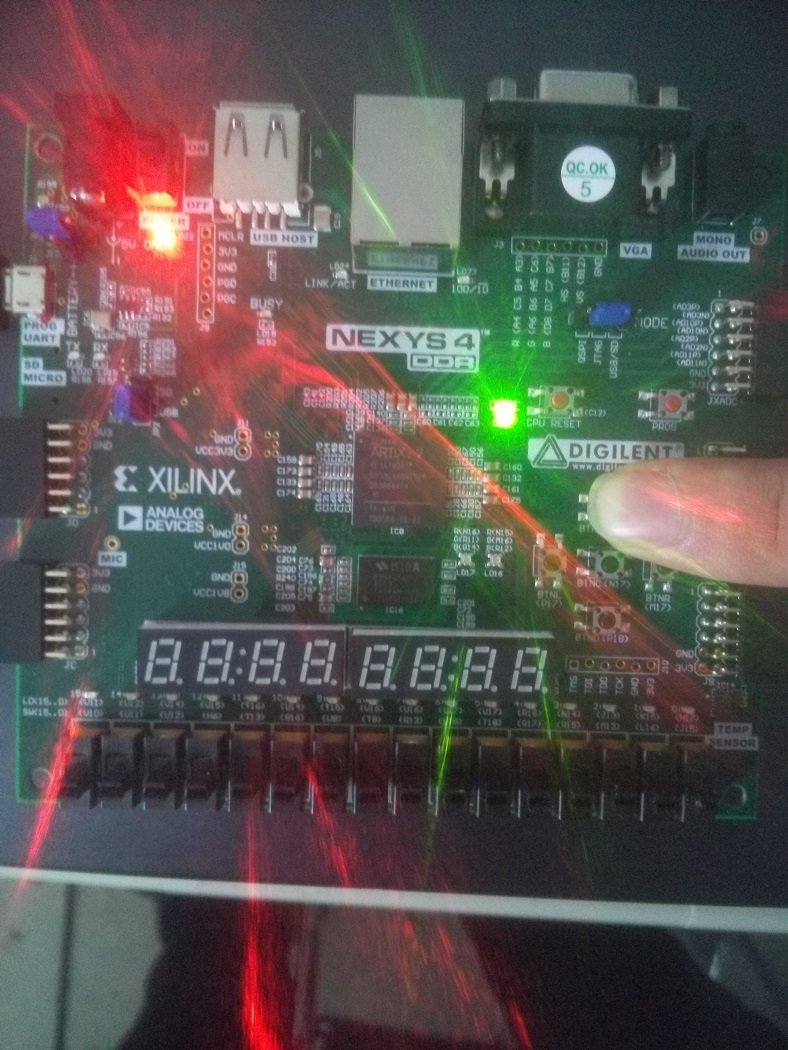
\includegraphics[width = 5in]{straight2.jpg}
  \end{center}
  
  \subsubsection*{左转}
  
  \begin{center}
    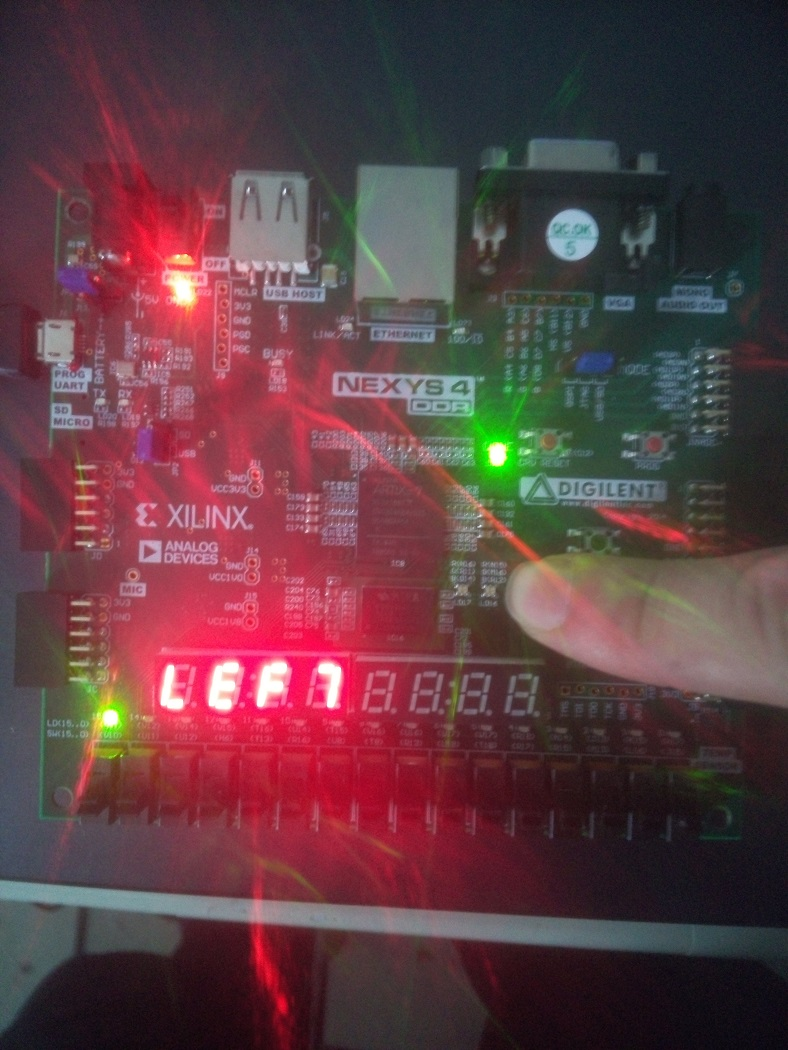
\includegraphics[width = 5in]{left2.jpg}
  \end{center}

  \subsubsection*{右转}

  \begin{center}
    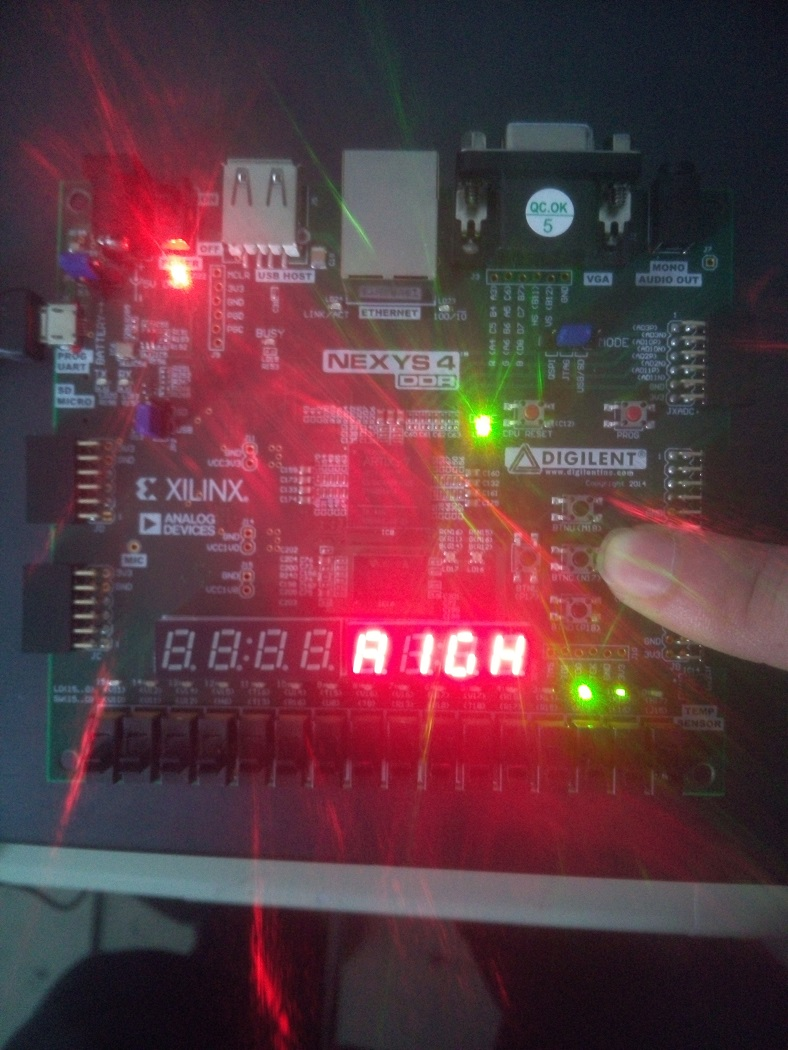
\includegraphics[width = 5in]{right2.jpg}
  \end{center}

  \subsubsection*{刹车}

  \begin{center}
    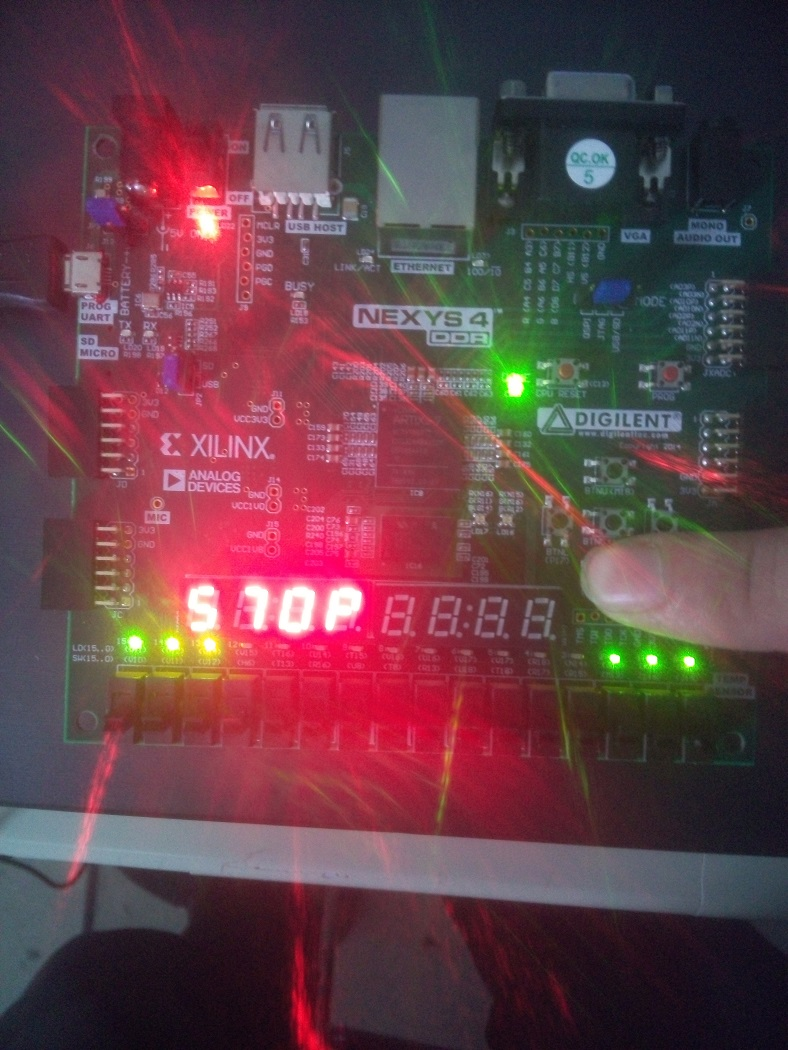
\includegraphics[width = 5in]{stop2.jpg}
  \end{center}

  \subsubsection*{错误}

  \begin{center}
    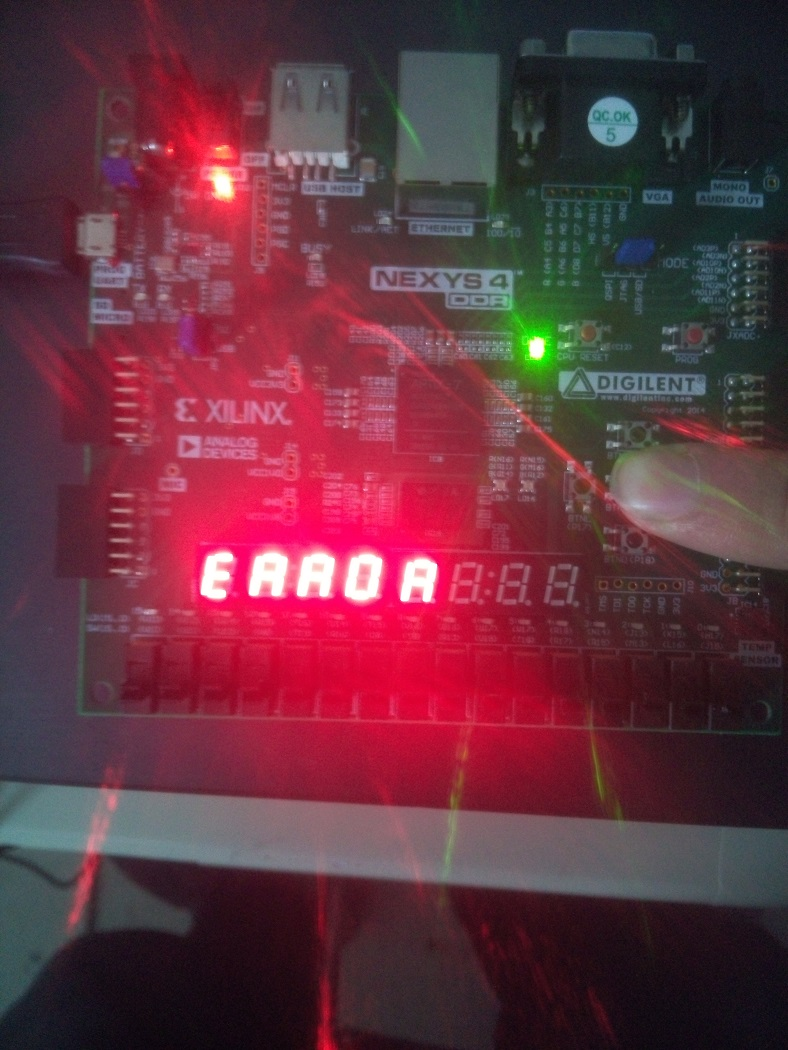
\includegraphics[width = 5in]{error2.jpg}
  \end{center}
  
  \subsection*{小组分工与合作}

  \addcontentsline{toc}{subsection}{附录四 \  小组分工与合作}

  由于我没有与其他同学组队,所以各项工作(包括资料查阅、总体设计、代码编写、程序调试)都由我一个人完成。
  
  \end{appendices}

  \section*{致谢}
  
  \addcontentsline{toc}{section}{致谢}

  感谢为一个小问题不惜亲自打电话的张英涛老师,让我认识到数字世界与为人师者的魅力。

  感谢数字逻辑设计实验课的助教,没有她们的教导,我不可能完成这项作业。
  
  \newpage
\end{CJK*}
\end{document}
